\documentclass[a4paper,10pt]{report}
\usepackage[cm]{fullpage}
\usepackage[utf8]{inputenc}
\usepackage{amsmath}
\usepackage{amsthm}
\usepackage{amssymb}
\usepackage{appendix}
\usepackage{booktabs}
\usepackage[table]{xcolor}
\usepackage{amssymb}
\usepackage{multirow}
\usepackage{fullpage}
\usepackage{float}
\usepackage{wrapfig}
\usepackage{subfig}
\usepackage{graphicx}
\usepackage{listings}
\usepackage{color}
\usepackage{textcomp}
\usepackage{sagetex}



\usepackage{hyperref}

\definecolor{listinggray}{gray}{0.9}
%\definecolor{lbcolor}{rgb}{0.9,0.9,0.9}

\addtolength{\voffset}{-10pt}

\hypersetup{colorlinks=false}
 
\lstset{
%	backgroundcolor=\color{lbcolor},
	tabsize=4,
%	rulecolor=,
	language=python,
        basicstyle=\scriptsize,
        upquote=true,
        aboveskip={1.5\baselineskip},
        columns=fixed,
        showstringspaces=false,
        extendedchars=true,
        breaklines=true,
        prebreak = \raisebox{0ex}[0ex][0ex]{\ensuremath{\hookleftarrow}},
%        frame=single,
        showtabs=false,
        showspaces=false,
        showstringspaces=false,
        identifierstyle=\ttfamily,
        keywordstyle=\color[rgb]{0,0,1},
        commentstyle=\color[rgb]{0.133,0.545,0.133},
        stringstyle=\color[rgb]{0.627,0.126,0.941},
} \hypersetup{colorlinks=false}

\renewcommand\chaptername{Esperimento}
 
\DeclareGraphicsExtensions{.pdf,.png,.jpg}


\author{Marco Giglio, Maria Cristina Fortuna, Riccardo Iaconelli}
% Title Page
\title{Relazioni dal Laboratorio di Fisica 2}

\begin{document}

\maketitle

\tableofcontents


%\chapter{Misura della velocità della luce}

L'obiettivo del nostro esperimento è misurare la velocità della luce $c$.

L'apparato di misurazione consiste principalmente in:
\begin{itemize}
 \item Un laser Elio-Neon ($\lambda=32$ nm).
 \item Uno specchio rotante a velocità angolare regolabile.
 \item Due lenti convergenti, di lunghezza focale $l_1 = 48mm$ e $l_2 = 252 mm$.
 \item Un microscopio con beam splitter e micrometro.
\end{itemize}

Lo specchio rotante viene fatto girare con velocità angolare $\omega_1$ in senso orario e $\omega_2$ in senso antiorario. Queste velocità angolari sono identiche nella maggior parte dei casi, e la loro differenza è trascurabile.

Chiamando $s_{cw}$ e $s_{ccw}$ rispettivamente le misure con specchio rotante in senso orario e antiorario, per come è orientata la strumentazione il numero
$$\Delta s = s_{cw} - s_{ccw}$$
deve essere positivo.

Purtroppo però non è questo il caso per qualche misura presa in mattinata, per ragioni sconosciute e che non siamo riusciti a riprodurre. Questi dati sono esclusi dalla misurazione in quanto evidenti errori, e sono mostrati in rosso nel grafico seguente
I dati sono molti, dunque forniamo qui soltanto una visione grafica, e lasciamo la tabella come allegato.

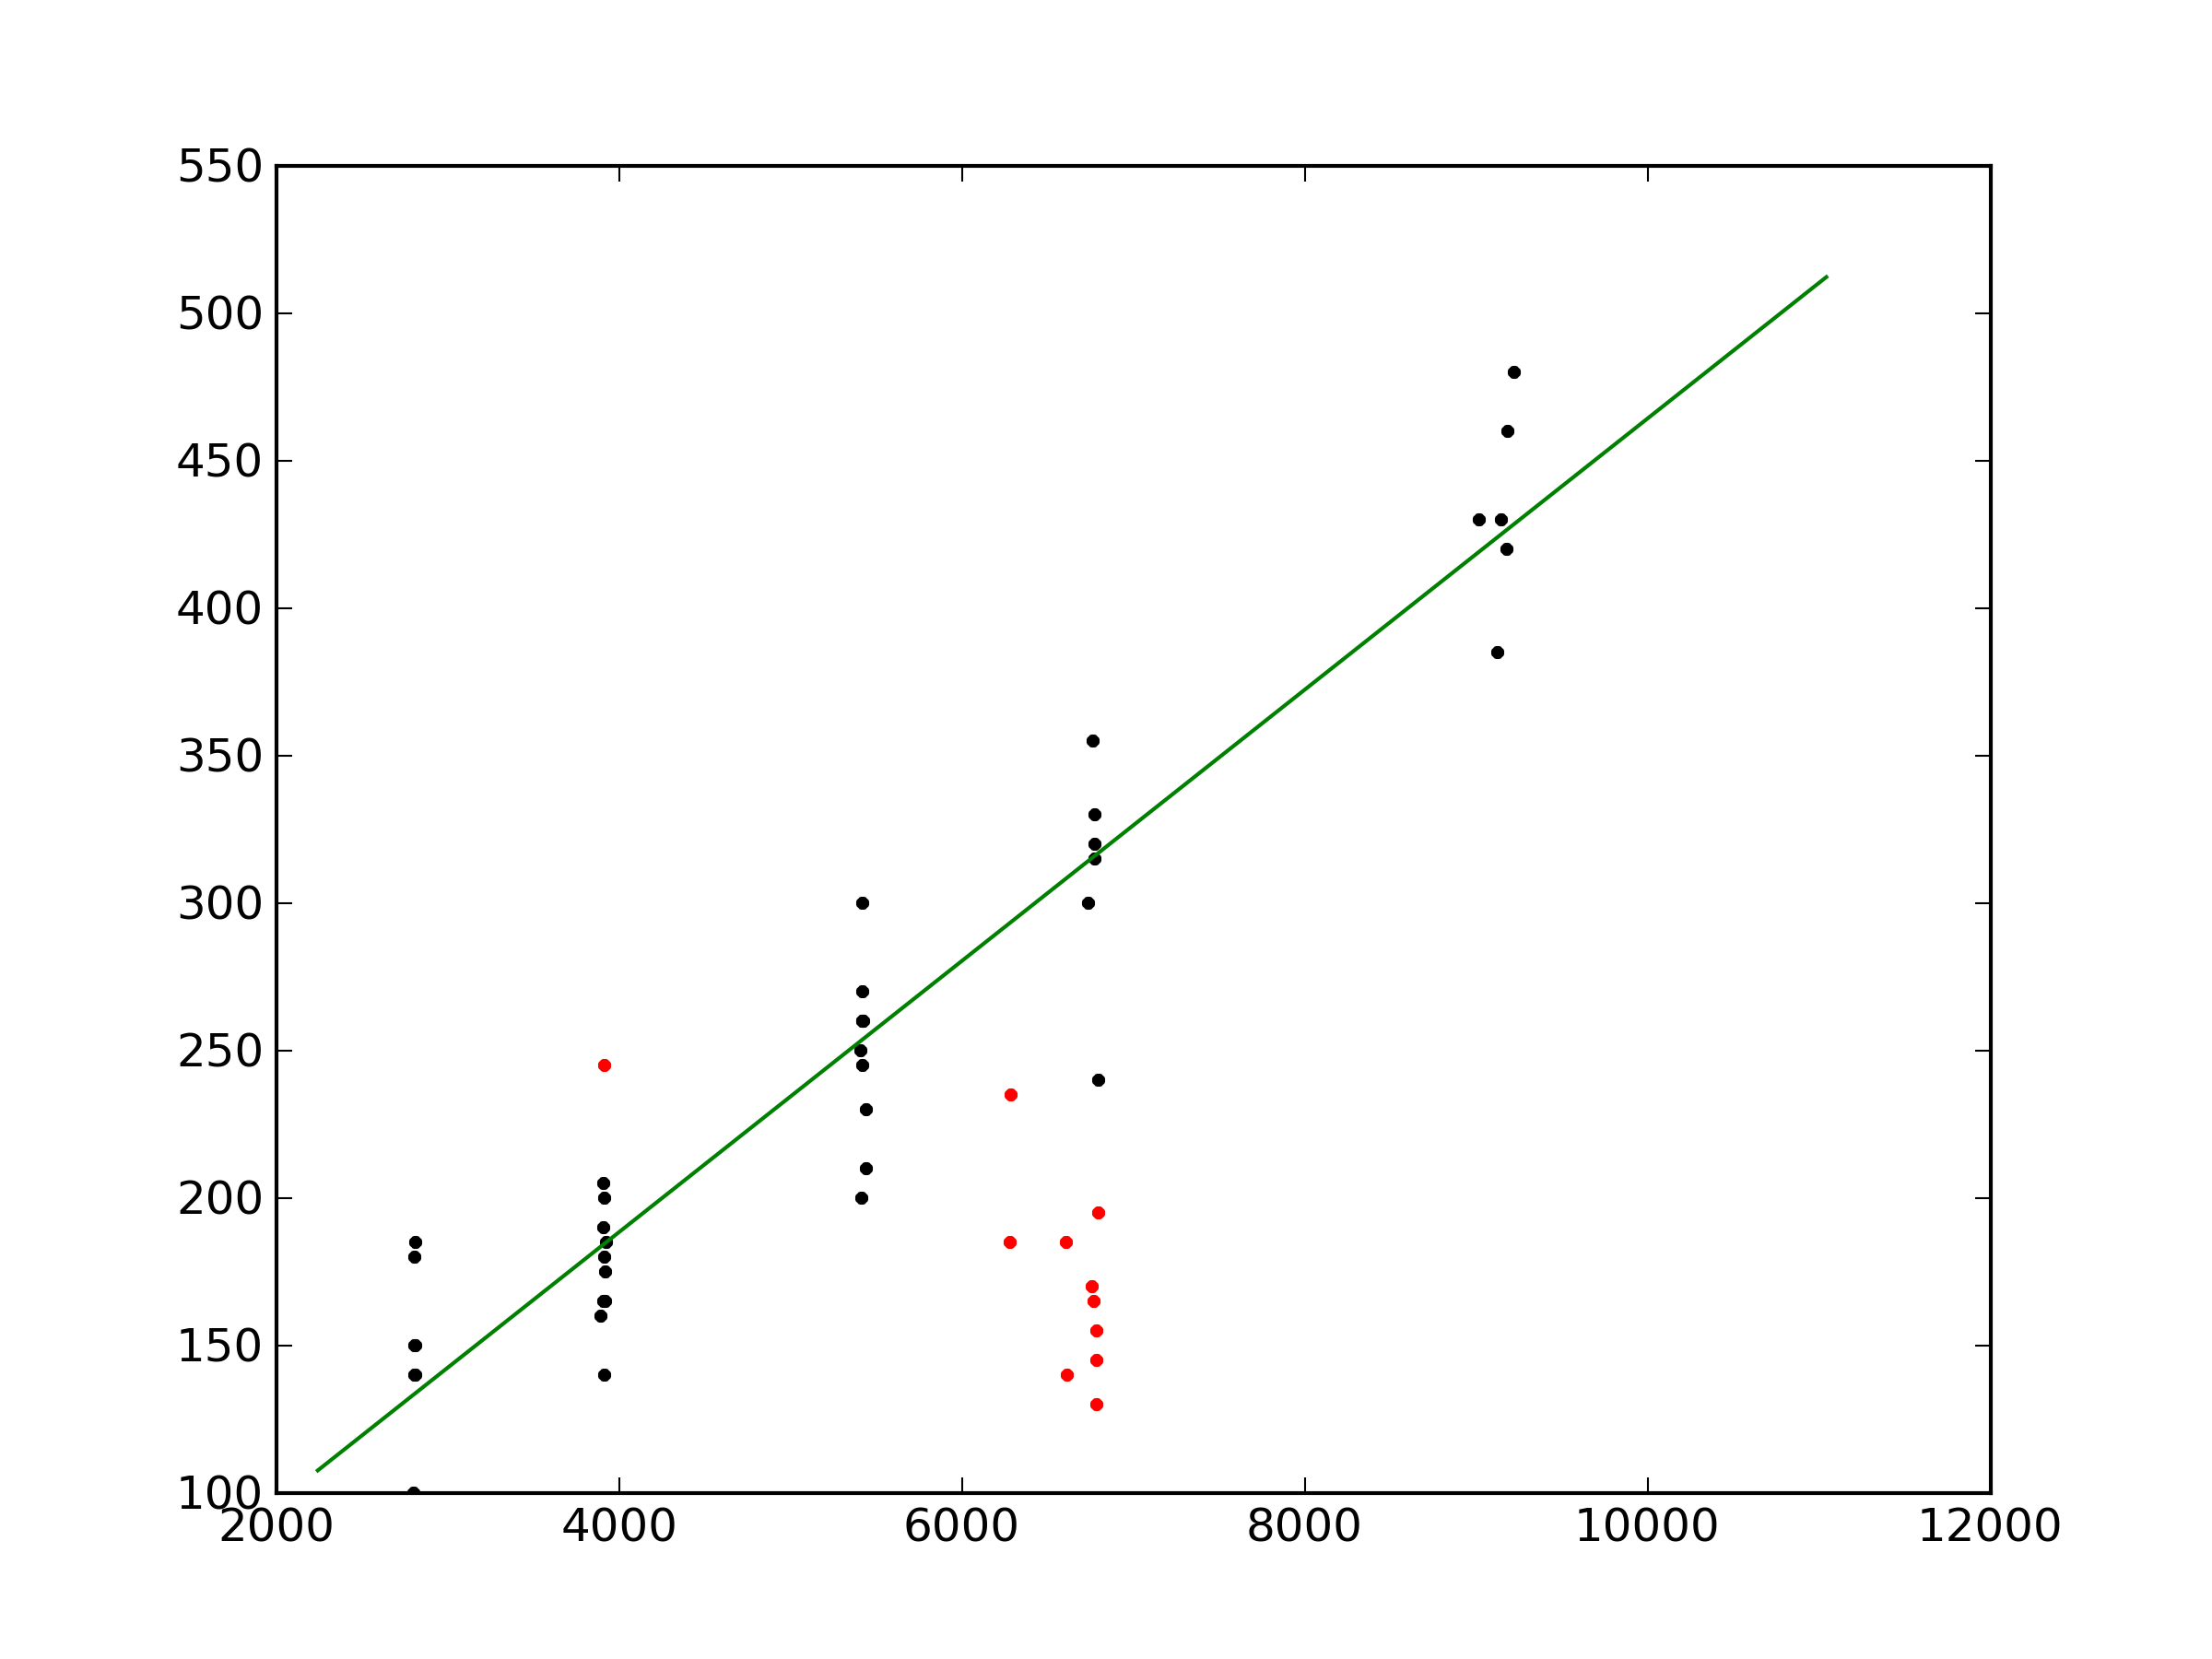
\includegraphics[scale=0.75]{grafici/C/dati.png}

\section{Analisi dati}

Chiamiamo $D = 13.480$m il cammino geometrico della luce per tornare allo specchio rotante, ovvero il doppio della distanza specchio rotante/specchio fisso; $A$ la distanza del punto di convergenza del fascio laser dalla lente $l_2$ e $B$ la distanza tra $l_2$ e lo specchio rotante. 

Per calcolare con precisione $A$, conoscendo la distanza focale di $l_2$, la ricaviamo dalla formula dei punti coniugati:
$$A=\frac{(B+D)f}{B+D-f} = 256\text{mm}$$


Per calcolare $c$, dobbiamo interpolare i dati presi nel modo seguente:
$$\Delta s = \frac{\tilde{A}}{c}\omega$$
ove
$$\tilde{A} = \frac{4*A*D^2}{2}$$

$\sage{2*e^2}$

La funzione che ci permetterà di calcolare $c$ è la seguente:

$$c = \frac{\tilde{A}}{m}$$
ove

Data una 
m=0.04594423946498933

Ricaviamo, tramite  il fit della funzione $V=R*I$" dove R è parametro da stimare, due resistenze ignote.


Misuro la resistenza interna del voltometro, mantenendo costante la ddp a $14.5\ V$ e variando la resistenza all'interno del circuito. 
Il voltmetro è in parallelo al circuito, perciò $R_i$:

$$R_i = \frac{RV}{RI-V} $$

dove R è la resistenza variabile, I la corrente nel circuito e $V= 14.5\ V$


La resistenza risulta $9.20 \pm 0.27 \ M \Omega$.


Misuriamo la resistenza interna dell'amperometro, che è collegato in serie al circuito. 

$$R_i = \frac{V-RI}{I}$$

In questo caso, R è fissato ($R=0.5 \Omega$) e sono V e I a variare

La resistenza interna risulta $11.42 \pm 0.45 \Omega$



Colleghiamo una piccola lampada a filamento al circuito, e verifichiamo che il suo comportamento resistivo non segue la legge di Ohm. 






%\chapter{Misura di resistenze}

L'obiettivo del nostro esperimento è misurare la validità della legge di Ohm per varie configurazioni di un circuito. 

Al fine di misurare corrente e potenziale, colleghiamo al nostro circuito due multimetri digitali. Il primo, che ha la funzione di voltmetro, lo poniamo ai capi della nostra resistenza collegato in parallelo; il secondo, in modalità amperometro, è posto in serie subito dopo la resistenza. 

Di seguito, gli strumenti con la loro precisione:
- Voltmetro (multimetro portatile), resistenza interna: 6 $M\Omega$
- Amperometro (multimetro da banco)
- Generatore da banco, resistenza interna ignota.


\section{Analisi dati}

Ricaviamo, tramite  il fit della funzione $V=R*I$" dove R è parametro da stimare, due resistenze ignote.

\subsection{Dati}

\begin{center}
\begin{tabular}{*{4}{c}}
Corrente1 & Potenziale1 & Corrente2 & Potenziale2\\
\midrule
396 & 201 & 3043 & 207\\
512 & 261 & 3667 & 250\\
706 & 360 & 4703 & 319\\
890 & 454 & 6365 & 432\\
1126 & 574 & 8984 & 609\\
1242 & 633 & 12326 & 836\\
1557 & 794 & 16898 & 1145\\
1812 & 925 & 340 & 24\\
1971 & 1005 & 725 & 50\\
2290 & 1168 & 966 & 66\\
2524 & 1286 & 1595 & 108\\
2850 & 1454 & 1822 & 124\\
3116 & 1589 & 2160 & 146\\
3407 & 1737 & 2302 & 157\\
3883 & 1980 & 2584 & 176\\
4229 & 2157 & 3100 & 211\\
4598 & 2344 & 3370 & 229\\
5072 & 2586 & 4036 & 274\\
5505 & 2807 & 4348 & 295\\
5820 & 2967 & 4596 & 312\\
6257 & 3191 & 4894 & 332\\
6738 & 3436 & 5578 & 379\\
7521 & 3835 & 6613 & 449\\
7880 & 4018 & 6963 & 473\\
8493 & 4331 & 7371 & 500\\
8852 & 4514 & 7864 & 533\\
9135 & 4658 & 8603 & 584\\
9431 & 4809 & 9066 & 615\\
9720 & 4957 & 9667 & 656\\
9972 & 5085 & 10816 & 733\\

\end{tabular}
\end{center}


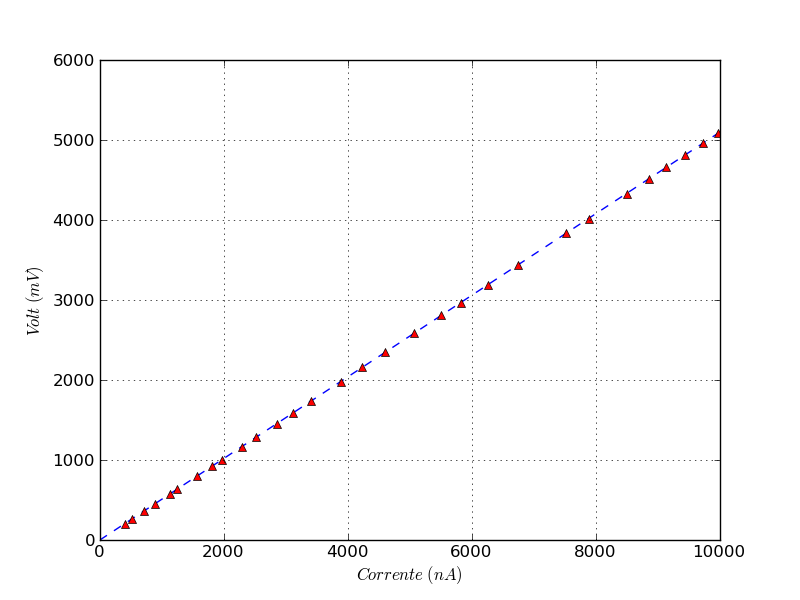
\includegraphics[scale=0.75]{grafici/C1/res1.png}
\
$\chi^2 = 5.76 $

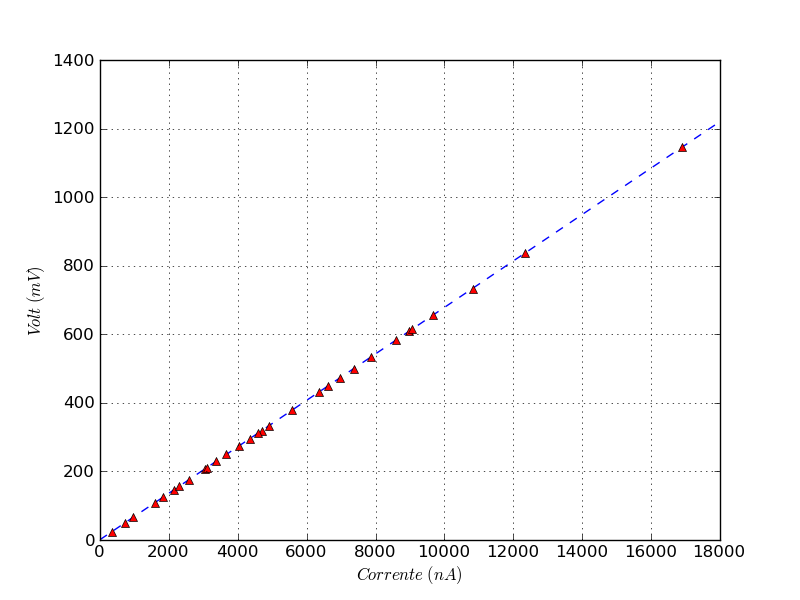
\includegraphics[scale=0.75]{grafici/C1/res2.png}

$\chi^2 = 4.88 $

Misuro la resistenza interna del voltometro, mantenendo costante la ddp a $14.5\ V$ e variando la resistenza all'interno del circuito. 
Il voltmetro è in parallelo al circuito, perciò $R_i$:

$$R_i = \frac{RV}{RI-V} $$

dove R è la resistenza variabile, I la corrente nel circuito e $V= 14.5\ V$

\begin{center}
\begin{tabular}{*{2}{c}}
Resistenza $M\Omega$ & Corrente $nA$\\
\midrule
7&      36\\
9&      32\\
10& 30\\
11&     29\\
12&     28\\
13&     27\\
14&     26\\
15&     26\\
16&     25\\
17&     24\\

\end{tabular}

La resistenza risulta $9.20 \pm 0.27 \ M \Omega$.


Misuriamo la resistenza interna dell'amperometro, che è collegato in serie al circuito. 

$$R_i = \frac{V-RI}{I}$$

In questo caso, R è fissato ($R=0.5 \Omega$) e sono V e I a variare
\begin{tabular}{*{2}{c}}
Volt $mV$ & Corrente $nA$\\
\midrule
22&      1769\\
40&      3271\\
60&      5047\\
105&     8938\\
133&     11201\\
142&     12021\\
164&     13882\\
174&     14745\\
208&     17604\\
232&     19671\\



\end{tabular}

La resistenza interna risulta $11.42 \pm 0.45 \Omega$


\end{center}


Colleghiamo una piccola lampada a filamento al circuito, e verifichiamo che il suo comportamento resistivo non segue la legge di Ohm. 

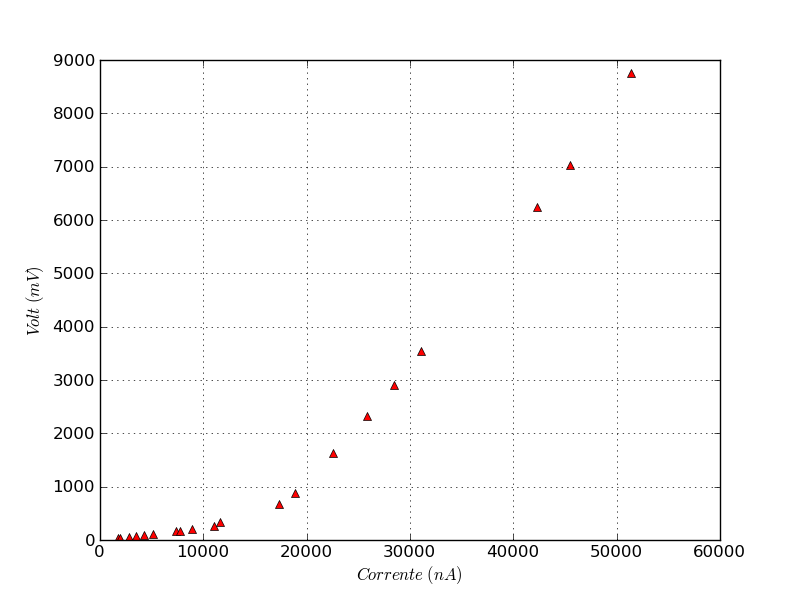
\includegraphics[scale=0.75]{grafici/C1/lampa.png}

La lampadina ha un comportamento non-ohmico nel momento in cui il filamento si scalda sufficientemente e inizia ad emettere luce ($500mV$).


\section{Partitore resistivo}

\subsection{Situazione senza carico}
\begin{center}
\begin{tabular}{*{2}{c}}
$V_{in}$ & $\frac{V_{in}}{V_{out}}$\\
\midrule
329.0 & 0.5015 \\
493.0 & 0.501 \\
544.0 & 0.5018 \\
618.0 & 0.5016 \\
667.0 & 0.5007 \\
776.0 & 0.5 \\
803.0 & 0.5006 \\
927.0 & 0.5005 \\
1078.0 & 0.5 \\
1285.0 & 0.4996 \\
\end{tabular}

\end{center}

$\chi^2=0.0169147373983$


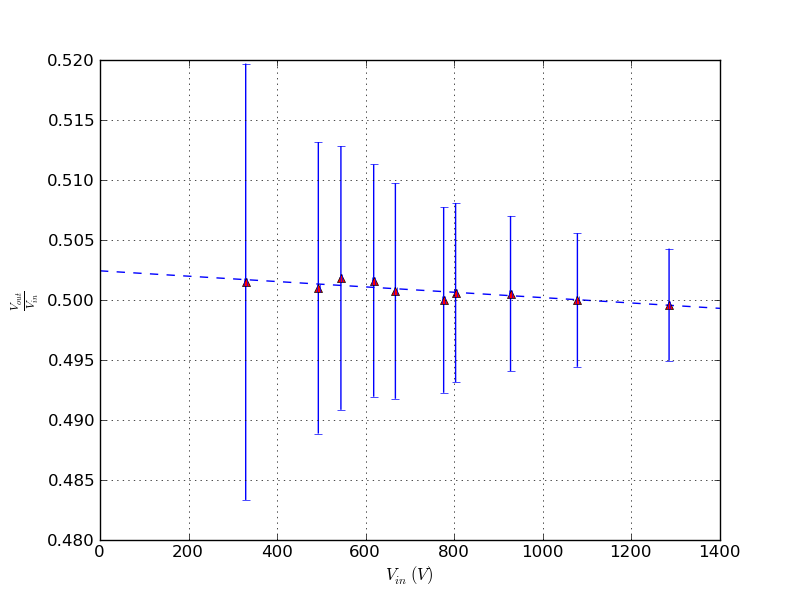
\includegraphics[scale=0.75]{grafici/C1/part1.png}

\subsection{Situazione con carico}
\begin{center}

\begin{tabular}{*{2}{c}}
$V_{in}$ & $\frac{V_{in}}{V_{out}}$\\
\midrule
220.0 & 3.1 \\
276.0 & 3.1051 \\
302.0 & 3.1126 \\
410.0 & 3.1073 \\
511.0 & 3.1115 \\
559.0 & 3.1055 \\
624.0 & 3.109 \\
752.0 & 3.109 \\
906.0 & 3.1093 \\
1036.0 & 3.111 \\
\end{tabular}

\end{center}
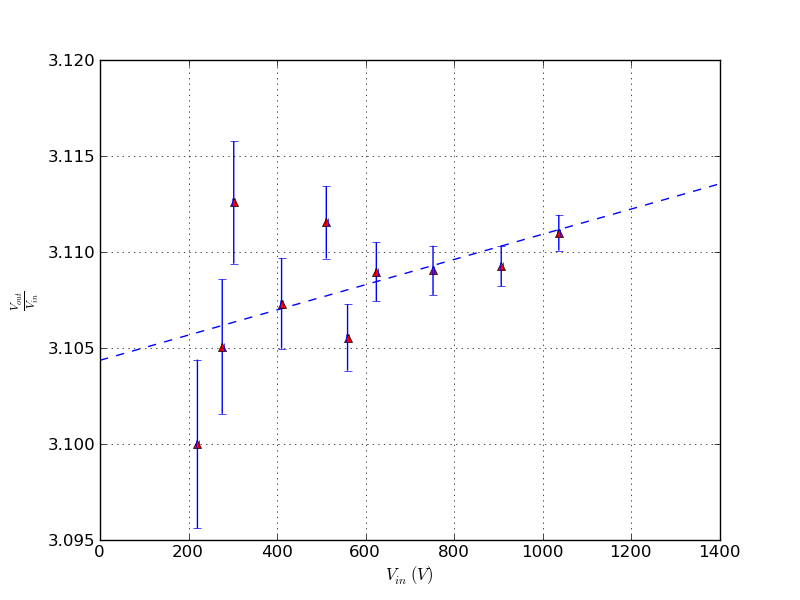
\includegraphics[scale=0.75]{grafici/C1/part2.png}

$\chi^2 = 12.9963702671$

\chapter{Circuiti RC e RL (C3)}

Oggetto di studio di questa esperienza è l'andamento della differenza di potenziale ai capi della resistenza e della capacità (o induttanza) di circuiti RC o RL in corrente impulsata e in corrente alternata.
A tal fine costruiamo un circuito con i seguenti elementi:

\begin{center}
 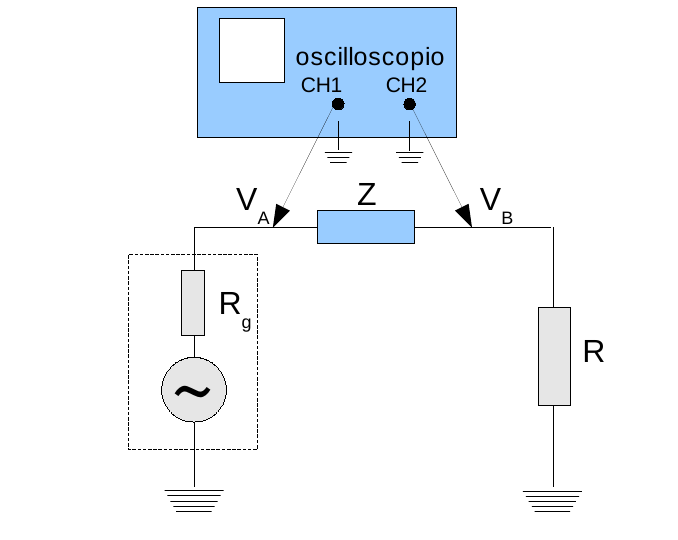
\includegraphics[scale=0.70]{grafici/C3/schema.png}
\end{center}

\begin{itemize}
  \item Generatore di onde di R= 50 $\Omega$
  \item Un condensatore di capacità 367 $nF$, misurata con il multimetro
  \item Un'induttore di induttanza sconosciuta, e resistenza 40 $\Omega$.
  \item Un oscilloscopio con due sonde
  \item Una resistenza di 677 $\Omega$ da noi misurata in C1 con un'incertezza che qui risulta trascurabile. 
\end{itemize}
La resistenza equivalente sul circuito è quindi:
\begin{itemize}
 \item Per il circuito RC: $R_{eq} = 677+50 = 727\ \Omega$.
 \item Per il circuito RL: $R_{eq} = 677+50+40 = 767\ \Omega$
\end{itemize}

\subsubsection{Nota sugli errori}
Tutte le misure di questa esperienza sono state effettuate osservando un display sul quale l'oscilloscopio rappresenta l'onda. La risoluzione (x,y) del display, dove x è l'asse temporale e y l'asse del potenziale, può essere variata a piacimento. 
Questo comporta una certa difficoltà nell'analisi degli errori. Per superarla, abbiamo notato che l'incertezza di ogni misura sulla misura stessa è un valore che rimane costante nel tempo, perchè abbiamo sempre cercato di non variare la dimensione dell'onda sullo schermo. Questo valore è tra il $4\%$ e l'$8\%$ del valore della singola misura. 


\section{Corrente impulsata: Studio del $\tau$ del circuito}

Per simulare l'apertura e la chiusura del circuito impostiamo nel generatore la modalità onda quadra. Colleghiamo la prima sonda all'ingresso del circuito, subito prima del condensatore: in tal modo l'oscilloscopio confronta il segnale in ingresso con la messa a terra, e visualizza a schermo la differenza di potenziale, restituendo sul display l'onda quadra prodotta dal generatore.  
Analogamente una seconda sonda, posta ai capi della resistenza, visualizza la forma dell'onda caratteristica della carica o della scarica del condensatore/induttore. \\
Raccogliamo i dati campionando dei punti dall'onda visualizzata sul display dell'oscilloscopio, usando i cursori per ottenere la ddp corrispondete all'istante di tempo considerato (si fissa il primo cursore sullo zero e il secondo sul punto dell'onda di cui si vuole conoscere il potenziale: l'oscilloscopio visualizza la differenza tra il potenziale dei due cursori, e dunque la ddp desiderata).
Infine interpoliamo i dati raccolti con le curve caratteristiche della carica per i due differenti circuiti, ricavando il parametro $\tau$ (tempo caratteristico dei circuiti).

\subsubsection{Circuito RC}
Con un'onda quadra a 50 Hz, abbiamo raccolto i seguenti dati:

\begin{center}
\begin{tabular}{*{2}{c}}
Tempo ($\mu s$) & Ddp ($V$) \\
\midrule
0 & 18.20 \\
100 & 12.80 \\
200 & 9.00 \\
300 & 5.80 \\
400 & 4.40 \\
500 & 3.20 \\
600 & 2.20 \\
700 & 1.80 \\
800 & 1.20 \\
900 & 1.00 \\
\end{tabular}
\end{center}

Interpoliamo i dati raccolti con la curva della carica di un condensatore: 
$$V_R = \varepsilon e^{-t/\tau}$$


%Tau per RC
\begin{sagesilent}

rct = np.recfromcsv('dati/C3/RCtau.csv')
tempo = rct['t']
volt = rct['v']
yerr = volt*0.08

def fu(P,x):
    return P[0]*exp((-1./P[1])*x)
    
def fu1(x,v,t):
    return v*exp(-x/t)
    
mymod = odr.Model(fu)
mydata = odr.RealData(tempo,volt)

myodr = odr.ODR(mydata, mymod, beta0=[20.,200.], maxit=5000)
out = myodr.run()

chi = chiquad(tempo,volt,fu1,ysigma=yerr,param=[out.beta[0],out.beta[1]])

chir = chi/(len(tempo)-2)
plt.clf()
plt.errorbar(tempo,volt,yerr,np.zeros_like(yerr),'ro')
xin = np.arange(0,1000,10)
yin = fu1(xin,out.beta[0],out.beta[1])
plt.plot(xin,yin,'--')
plt.ylabel(r"$D.d.p$ $(V)$ ")
plt.xlabel(r"$Tempo$ $(\mu s)$")
plt.grid(True)
plt.savefig("grafici/C3/RCtau.png",dpi=300)

\end{sagesilent}


\begin{center}
 \includegraphics[scale=0.70]{grafici/C3/RCtau.png}
\end{center}

Il valore stimato dall'interpolazione è $\tau=\sage{round(out.beta[1],2)}\pm \sage{round(out.sd_beta[1],2)}\ \mu s$.
Valore atteso: $\tau=RC=266.8\ \mu s$, con R=$727\ \Omega$.
L'errore è l'incertezza della misura del tempo e del potenziale, letti sul display dell'oscilloscopio. Per quanto riguarda il tempo, l'errore è stata assunto trascurabile poichè abbiamo campionato usando la griglia dell'oscilloscopio; per quanto riguarda il potenziale, abbiamo stimato un'errore percentuale del 8\%, che è circa il rapporto tra l'incertezza dello strumento e il valore della misura. 
\\
Per verificare l'accordo tra la legge e la distribuzione dei valori osservati operiamo il test del $\chi^2$:

Otteniamo $\chi^2 = \sage{round(chi,3)}$ con d.o.f = $\sage{len(tempo)-1}$\\
Il p-value associato è $0.066$, maggiore della soglia di accettabilità di $0.05$.

\subsubsection{Circuito RL}
Con un'onda quadra a 250 Hz, abbiamo raccolto i seguenti dati:

\begin{center}
\begin{tabular}{*{2}{c}}
Tempo ($\mu s$) & Ddp ($V$) \\
\midrule
5 & 5.00 \\
10 & 8.00 \\
15 & 10.60 \\
20 & 12.40 \\
25 & 13.60 \\
30 & 14.60 \\
35 & 15.40 \\
40 & 16.20 \\
45 & 16.40 \\
\end{tabular}
\end{center}
Interpoliamo i dati raccolti con la curva caratteristica della carica del circuito:

$$V_R = \varepsilon \left( 1-e^{-t/\tau} \right)$$

%Tau per RL
\begin{sagesilent}
 
rlt = np.recfromcsv('dati/C3/RLtau.csv')
tempo = rlt['t']
volt = rlt['v']
yerr = volt*0.04

def fu(P,x):
    return P[0]*(1-exp((-1./P[1])*x))
    
def fu1(x,v,t):
    return v*(1-exp(-x/t))
    
mymod = odr.Model(fu)
mydata = odr.RealData(tempo,volt)

myodr = odr.ODR(mydata, mymod, beta0=[20.,16.], maxit=5000)
out = myodr.run()

chi = chiquad(tempo,volt,fu1,ysigma=yerr,param=[out.beta[0],out.beta[1]])
dof = len(tempo)-2
chir = chi/dof

plt.clf()
plt.errorbar(tempo,volt,yerr,np.zeros_like(yerr),fmt=None)
plt.plot(tempo,volt,'ro')
xin = np.arange(min(tempo),1.5*max(tempo),1)
yin = fu1(xin,out.beta[0],out.beta[1])
plt.plot(xin,yin,'b--')
plt.ylabel(r"$D.d.p$ $(V)$ ")
plt.xlabel(r"$Tempo$ $(\mu s)$")
plt.grid(True)
plt.savefig("grafici/C3/RLtau.png",dpi=300)

\end{sagesilent}




\begin{center}
 \includegraphics[scale=0.70]{grafici/C3/RLtau.png}
\end{center}

Il valore stimato dall'interpolazione è $\tau=\sage{round(out.beta[1],2)} \pm \sage{round(out.sd_beta[1],2)}\ \mu s$. Il fit ha un $\chi^2 = \sage{round(chi,2)} $ con $d.o.f= \sage{dof}$. Il p-value associato è $0.83$.
\\

Valgono le considerazioni precedenti per quanto riguarda le incertezze. 

\section{Corrente alternata: studio frequenza di taglio}

Nella seconda parte dell'esperienza intendiamo misurare la risposta in frequenza (o funzione di trasferimento).

Pertanto misuriamo la ddp ai capi di $R$ e $C$ o $L$ in modo analogo alle prima parte dell'esperienza, e la distanza tra due picchi delle onde visualizzate a schermo per determinare l'angolo $\phi$ di sfasamento ($\delta \phi = 2 \pi \Delta t$).

Per ricavare il rapporto $\frac{V_{R}}{V_{o}}$, dobbiamo ricavare $V_R$. Trovandoci in regime di corrente alternata, la leggge di Ohm è nella forma: $ V_o = Zi_o$ con $Z = R + jX$, impedenza del circuito.
Trattandosi di circuiti RC e RL in cui le impedenze sono collegate in serie, si ha $Z_{tot} = \sum Z_i$

\begin{itemize}
\item circuito RC: $Z=R-\frac{j}{\omega C}$
\item circuito RL: $Z=R+j\omega L$
\end{itemize}  

Allora otteniamo la coppia di equazioni 

$$V_{Ro} = Ri_o = \frac{V_o}{Z} = \frac{RV_o}{\sqrt{R^2+X^2}} $$ 

$$\phi = \arctan \frac{X}{R} $$


Dove ad $X$ sostituiamo:
\begin{itemize}
\item Per il circuito RC: $X=\frac{1}{\omega C}$
\item Per il circuito RL: $X=\omega L$
\end{itemize}

Per ricavare l'opportuna funzione di trasferimento.

\subsection*{Circuito RC}


\begin{center}

\begin{tabular}{*{4}{c}}
Frequenza ($Hz$) & $V_{out}/V_{in}$ & $\phi\ (rad))$ & Delta ($\mu s$)\\
\midrule
50 & 0.08 & 1.54 & 4900\\
100 & 0.15 & 1.41 & 2240\\
200 & 0.30 & 1.41 & 1120\\
300 & 0.42 & 1.24 & 660\\
400 & 0.52 & 1.08 & 430\\
1000 & 0.83 & 0.70 & 112\\
1500 & 0.90 & 0.49 & 52\\
2000 & 0.93 & 0.38 & 30\\
4000 & 0.97 & 0.20 & 8\\

\end{tabular}
\end{center}

Lasciamo C come parametro da stimare, e interpoliamo i valori raccolti di $V_{out}$ e $V_{in}$ in funzione della frequenza, usando l'equazione:

$$\frac{V_{Ro}}{V_o} = \frac{R}{\sqrt{R^2+(\omega C)^{-2}}}$$

dove $V_{Ro} = V_{out}$ (tensione ai capi della resistenza) e $V_o = V_{in}$.

%Fit DDP per RC
\begin{sagesilent}

rcf = np.recfromcsv('dati/C3/RCfun.csv')
freq = rcf['frequenza']
freq = freq.astype(float)
vin= rcf['v_in']
volt = rcf['v_out']/rcf['v_in']
yerr = 0.01
xerr = 0

var('x,C')
def funz(x, C):
    return 727/sqrt(727^2+(x*2*n(pi)*C)^(-2))
    
def func(P,x):
    return 727/sqrt(727^2+(x*2*n(pi)*P[0])^(-2))
    
mymod = odr.Model(func)
mydata = odr.RealData(freq,volt)

myodr = odr.ODR(mydata, mymod, beta0=[0.0000001], maxit=5000)
out = myodr.run()

chi = chiquad(freq,volt,funz,ysigma=float(yerr),param=[out.beta[0]])

chir = chi/(len(freq)-1)

omega = 1/((727)*out.beta[0])
 
plt.clf()

xin = np.arange(min(freq),1.5*max(freq),10)
yin = funz(xin,out.beta[0])
plt.semilogx(freq,volt,'ro')
plt.errorbar(freq,volt,yerr,xerr,fmt=None)
plt.plot(xin,yin,'b--')
plt.ylabel(r"$\frac{V_{out}}{V_{in}}$ ")
plt.xlabel(r"$\nu$ Frequenza $(Hz)$")
plt.grid(True)
plt.savefig("grafici/C3/RCddp.png",dpi=300)
 
\end{sagesilent}


\begin{center}
 \includegraphics[scale=0.70]{grafici/C3/RCddp.png}
\end{center}

Dal fit otteniamo $C=365.42 \pm  6.11\ nF $, un $\chi^2 = \sage{round(chi,3)}$ con $d.o.f=\sage{len(freq)-1}$ e p-value: 0.25 

La frequenza di taglio è definita come $\omega_c = \frac{1}{RC}$ e per questo valore di C otteniamo $\omega_c = \sage{round(omega,2)}\ Hz$.

L'errore $\sigma_v$ deriva dagli errori su $V_{out}$ e $V_{in}$:

$\sigma_V = \sqrt{\frac{\sigma_{out}^2}{V_{in}^2} + \frac{\sigma_{in}^2}{V_{in}^4} }$

Per questa formula di propagazione, l'errore risulta irrilevante, e abbiamo stimato un'errore di $0.01 V$.
%Fit Phi per RC
\begin{sagesilent}

deltaphi= rcf['frequenza']*rcf['tempo']*2*n(pi)*10^(-6)
yerr = deltaphi*0.06
xerr= 0

var('x,C')
def funz(x, C):
    return arctan(1/(x*2*n(pi)*727*C))
    
def func(P,x):
    return arctan(1/(x*2*n(pi)*727*P[0]))
    
mymod = odr.Model(func)
mydata = odr.RealData(freq,deltaphi)

myodr = odr.ODR(mydata, mymod, beta0=[0.0000001], maxit=5000)
out = myodr.run()

chi = chiquad(freq,deltaphi,funz,ysigma=yerr,param=[out.beta[0]])

chir = chi/(len(freq)-1)

ddof=len(freq)-len(out.beta) 
 
plt.clf()

xin = np.arange(min(freq),1.5*max(freq),10)
yin = funz(xin,out.beta[0])
plt.semilogx(freq,deltaphi,'ro')
plt.errorbar(freq,deltaphi,yerr,xerr,fmt=None)
plt.plot(xin,yin,'b--')
plt.ylabel(r"$\phi (rad)$ ")
plt.xlabel(r"$\nu$ Frequenza $(Hz)$")
plt.grid(True)
plt.savefig("grafici/C3/RCfase.png",dpi=300)

omega = 1/(727*out.beta[0])
out.pprint()

\end{sagesilent}


Ora interpolo i dati della $ \phi$ utilizzando la funzione:

$$ \phi = \arctan \frac{1}{2\pi\nu C R} $$


\begin{center}
 \includegraphics[scale=0.70]{grafici/C3/RCfase.png}
\end{center}


Ricavo $C=264.90 \pm 10.1\ nF$.
Ottengo un $\chi^2 = \sage{round(chi,3)}$ con $d.o.f= \sage{len(deltaphi)-1}$ e p-value $=\sage{round(chdtrc(ddof,float(chi)),3)}$
L'errore su y è $\sigma_{y_i} = 2 \pi \nu_i \sigma_{t}$. Abbiamo supposto $\sigma_{t}$ proporzionale al tempo (è l'incertezza sulla lettura) e pari al $6\%$.
Per questo secondo valore di C, $\omega_c = \sage{round(omega,2)}\ Hz$. 

\subsubsection{Considerazioni teoriche}
Il comportamento del circuito varia a seconda di quanto la nostra frequenza $\omega$ si avvicina al valore della frequenza di taglio. \\
Per frequenze molto basse il carattere capacitivo dell'impedenza domina e pertanto la caduta di potenziale si trova tutta ai capi del condensatore, e la fase $\phi \simeq -\frac{\pi}{2}$. Viceversa per frequenze molto alte, domina il comportamento resistivo e lo sfasamento diviene: $ \phi \simeq 0$. \\  
Per $\omega \simeq \omega_c$, siamo nella transizione tra i due regimi e le impedenze si equivalgono. La fase diviene: $ \phi \simeq -\pi/4$.  \\

L'insieme dei fenomeni da noi osservati in questa secondo parte, ci permette di affermare che il circuito RC da noi costruito agisce come un filtro passa-basso passivo, cioè un filtro che riduce le componenti alle frequenze superiori a quella di taglio (abbattendo l'ampiezza di $V_{out}$ all'aumentare della frequenza, come si vede nel grafico). Il più semplice filtro passa-basso è, infatti, un circuito RC. 

\subsection*{Circuito RL}
\begin{center}

\begin{tabular}{*{4}{c}}
Frequenza ($Hz$) & Delta V ($V_{out}/V_{in}$) & $\phi (rad)$ & Delta ($\mu s$) \\
\midrule
1000& 0.47 & 0.19 & 30 \\
2000 & 0.62 & 0.35 & 28\\
3000 & 0.79 & 0.45 & 24\\
4000 & 1.05 & 0.58 & 23\\
6000 & 1.48 & 0.79 & 21\\
8000 & 2.01 & 1.01 & 20\\
10000 & 2.56 & 0.94 & 15\\
15000 & 3.64 & 1.13 & 12\\
20000 & 4.28 & 1.26 & 10 \\
30000 & 5.08 & 1.36 & 7.2\\
50000 & 5.89 & 1.57 & 5\\
\end{tabular}
\end{center}



Anche questa volta interpoliamo i dati raccolti con la funzione:

$$\frac{V_{Ro}}{V_o} = \frac{R}{\sqrt{R^2+(\omega L)^2}}$$


%Fit DDP per RL
\begin{sagesilent}

#Fit del ddp in funzione della frequenza per l'induttore
dati3 = np.recfromcsv('dati/C3/RLfun.csv',delimiter="\t")
dati3 = np.sort(dati3)

deltaV = dati3['v_out']/dati3['v_in']
yerr = 0.05
xerr= 0

var('x,L')

def func(x, L):
    return (767/(np.sqrt((767)^2+(x*2*n(pi)*L)^2)))

def fu(P, x):
    return func(x, P[0])
 
import scipy.odr as odr
mymodel = odr.Model(fu)
mydata = odr.RealData(dati3['frequenza'], deltaV)
myodr = odr.ODR(mydata, mymodel, beta0=[0.002],  maxit=1000)
myout = myodr.run()

chiquadrato = chiquad(np.array(dati3['frequenza']), deltaV, fu, ysigma=float(0.1), param=[myout.beta])

plt.clf()
plt.semilogx(dati3['frequenza'],deltaV , 'ro')
xsp = np.arange(0, 500000, 500)
ysp = func(xsp, myout.beta[0])
plt.plot(xsp, ysp, 'b--')
plt.errorbar(dati3['frequenza'],deltaV,yerr,xerr,fmt=None)
plt.grid(True)
plt.ylabel(r"$\frac{V_{out}}{V_{in}}$ ")
plt.xlabel(r"Frequenza $\nu$ - $(Hz)$")
plt.savefig("grafici/C3/RLddp.png", dpi=300)
omega = 767/myout.beta[0]
lstring = "%.4G" % (myout.beta[0]*1000)
lerrorstring = "%.2G" % (myout.sd_beta[0]*1000)
\end{sagesilent}

\begin{center}
 \includegraphics[scale=0.70]{grafici/C3/RLddp.png}
\end{center}



Otteniamo $L=\sage{lstring}\pm\sage{lerrorstring} \ H$.  Non ha senso calcolare il $\chi^2$, poichè la funzione di fit non è in buon accordo con i nostri dati. Sospettiamo la presenza di impedenze ignote che abbiamo trascurato.


La frequenza di taglio viene definita come $\omega_c = R/L$. Usando la L di questo fit, $\omega_c = \sage{round(omega,2)}\ Hz$. 

%Fit Phi per RL
\begin{sagesilent}

rlf = np.recfromcsv('dati/C3/RLfun.csv',delimiter="\t")
freq = rlf['frequenza']
deltaphi= rlf['frequenza']*rlf['delta']*2*n(pi)*10^(-6)
yerr = deltaphi*0.06
xerr= 0

var('x,L')
def funz(x, L):
    return arctan(x*2*n(pi)*L/767)
    
def func(P,x):
    return arctan(x*2*n(pi)*P[0]/767)
    
mymod = odr.Model(func)
mydata = odr.RealData(freq,deltaphi)

myodr = odr.ODR(mydata, mymod, beta0=[0.012], maxit=1000)
out = myodr.run()

chi = chiquad(freq,deltaphi,funz,ysigma=yerr,param=[out.beta[0]])

chir = chi/(len(freq)-1)
 
plt.clf()

xin = np.arange(0.5*min(freq),1.5*max(freq),10)
yin = funz(xin,out.beta[0])
plt.semilogx(freq,deltaphi,'ro')
plt.errorbar(freq,deltaphi,yerr,xerr,fmt=None)
plt.plot(xin,yin,'b--')
plt.ylabel(r"$\phi (rad)$ ")
plt.xlabel(r"$\nu$ Frequenza $(Hz)$")
plt.grid(True)
plt.savefig("grafici/C3/RLfase.png",dpi=300)
out.pprint()
omega = 767/(out.beta[0])

\end{sagesilent}


Interpolo i dati della $\phi$, utilizzando la funzione:

$$ \phi = \arctan \frac{2\pi\nu L}{R} $$

dove L è il parametro libero da stimare.

\begin{center}
 \includegraphics[scale=0.70]{grafici/C3/RLfase.png}
\end{center}


$L=20.2\pm0.01\ mH$. Il fit ha un $\chi^2 = \sage{round(chi,2)}$ con $d.o.f= \sage{len(freq)-1}$ e p-value:0.18. Per l'analisi degli errori, valgono le considerazioni fatte in precedenza per il circuito RC.\\

La frequenza di taglio viene definita come $\omega_c = R/L$. Usando la L di questo fit, $\omega_c = \sage{round(omega,2)}\ Hz$. 
\\
\subsubsection{Considerazioni teoriche}
Il comportamento del nostro circuito varia a seconda di quanto la nostra frequenza $\omega$ si avvicina al valore della frequenza di taglio. \\
Per frequenze molto basse il carattere resistivo dell'impedenza domina e pertanto la caduta di potenziale si trova solo ai capi della resistenza; per cui $ \phi \simeq 0$. Viceversa per frequenze molto alte, domina il comportamento induttivo, e lo sfasamento prodotto è simile a quello che introdurrebbe nel circuito un componente puramente induttivo ($\phi \simeq \frac{\pi}{2}$).  \\
Per $\omega = \omega_c$, essendo in transizione tra i due regime, si ha un comportamento intermedio e la fase diviene: $ \phi = \pi/4$. \\

L'insieme dei fenomeni da noi osservati in questa secondo parte, ci permette di affermare che il circuito RL da noi costruito agisce come un filtro passa-alto passivo, cioè un filtro che riduce le componenti alle frequenze inferiori a quella di taglio (abbattendo l'ampiezza di $V_{out}$ al diminuire della frequenza , come si vede nel grafico). Il più semplice filtro passa-alto è, infatti, un circuito RL. 

%\chapter{Misura di resistenze}

L'obiettivo del nostro esperimento è misurare la validità della legge di Ohm per varie configurazioni di un circuito. 

Al fine di misurare corrente e potenziale, colleghiamo al nostro circuito due multimetri digitali. Il primo, che ha la funzione di voltmetro, lo poniamo ai capi della nostra resistenza collegato in parallelo; il secondo, in modalità amperometro, è posto in serie subito dopo la resistenza. 

Di seguito, gli strumenti con la loro precisione:
- Voltmetro (multimetro portatile), resistenza interna: 6 $M\Omega$
- Amperometro (multimetro da banco)
- Generatore da banco, resistenza interna ignota.


\section{Analisi dati}

Ricaviamo, tramite  il fit della funzione $V=R*I$" dove R è parametro da stimare, due resistenze ignote.

\subsection{Dati}

\begin{center}
\begin{tabular}{*{4}{c}}
Corrente1 & Potenziale1 & Corrente2 & Potenziale2\\
\midrule
396 & 201 & 3043 & 207\\
512 & 261 & 3667 & 250\\
706 & 360 & 4703 & 319\\
890 & 454 & 6365 & 432\\
1126 & 574 & 8984 & 609\\
1242 & 633 & 12326 & 836\\
1557 & 794 & 16898 & 1145\\
1812 & 925 & 340 & 24\\
1971 & 1005 & 725 & 50\\
2290 & 1168 & 966 & 66\\
2524 & 1286 & 1595 & 108\\
2850 & 1454 & 1822 & 124\\
3116 & 1589 & 2160 & 146\\
3407 & 1737 & 2302 & 157\\
3883 & 1980 & 2584 & 176\\
4229 & 2157 & 3100 & 211\\
4598 & 2344 & 3370 & 229\\
5072 & 2586 & 4036 & 274\\
5505 & 2807 & 4348 & 295\\
5820 & 2967 & 4596 & 312\\
6257 & 3191 & 4894 & 332\\
6738 & 3436 & 5578 & 379\\
7521 & 3835 & 6613 & 449\\
7880 & 4018 & 6963 & 473\\
8493 & 4331 & 7371 & 500\\
8852 & 4514 & 7864 & 533\\
9135 & 4658 & 8603 & 584\\
9431 & 4809 & 9066 & 615\\
9720 & 4957 & 9667 & 656\\
9972 & 5085 & 10816 & 733\\

\end{tabular}
\end{center}


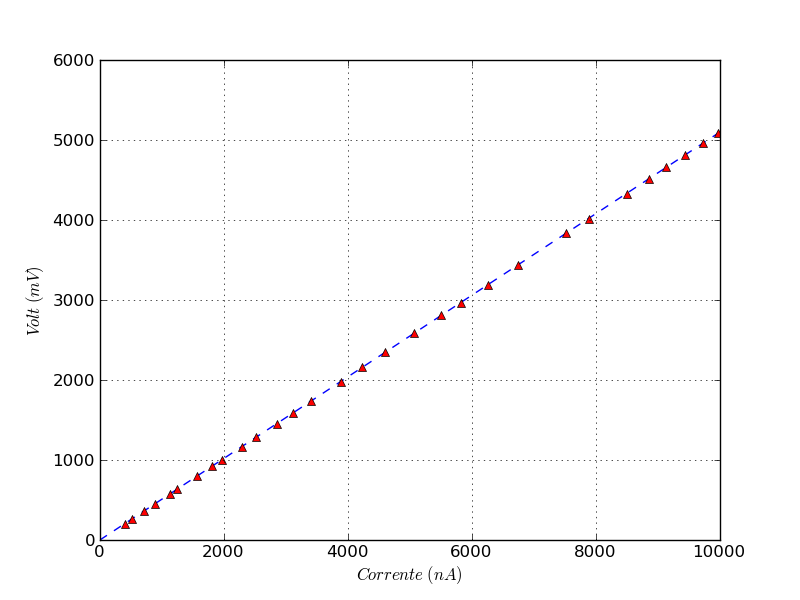
\includegraphics[scale=0.75]{grafici/C1/res1.png}
\
$\chi^2 = 5.76 $

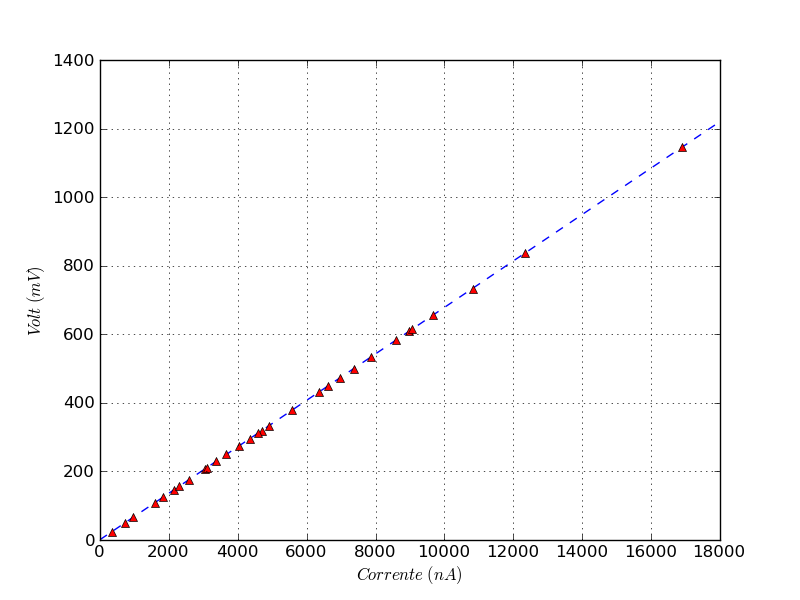
\includegraphics[scale=0.75]{grafici/C1/res2.png}

$\chi^2 = 4.88 $

Misuro la resistenza interna del voltometro, mantenendo costante la ddp a $14.5\ V$ e variando la resistenza all'interno del circuito. 
Il voltmetro è in parallelo al circuito, perciò $R_i$:

$$R_i = \frac{RV}{RI-V} $$

dove R è la resistenza variabile, I la corrente nel circuito e $V= 14.5\ V$

\begin{center}
\begin{tabular}{*{2}{c}}
Resistenza $M\Omega$ & Corrente $nA$\\
\midrule
7&      36\\
9&      32\\
10& 30\\
11&     29\\
12&     28\\
13&     27\\
14&     26\\
15&     26\\
16&     25\\
17&     24\\

\end{tabular}

La resistenza risulta $9.20 \pm 0.27 \ M \Omega$.


Misuriamo la resistenza interna dell'amperometro, che è collegato in serie al circuito. 

$$R_i = \frac{V-RI}{I}$$

In questo caso, R è fissato ($R=0.5 \Omega$) e sono V e I a variare
\begin{tabular}{*{2}{c}}
Volt $mV$ & Corrente $nA$\\
\midrule
22&      1769\\
40&      3271\\
60&      5047\\
105&     8938\\
133&     11201\\
142&     12021\\
164&     13882\\
174&     14745\\
208&     17604\\
232&     19671\\



\end{tabular}

La resistenza interna risulta $11.42 \pm 0.45 \Omega$


\end{center}


Colleghiamo una piccola lampada a filamento al circuito, e verifichiamo che il suo comportamento resistivo non segue la legge di Ohm. 

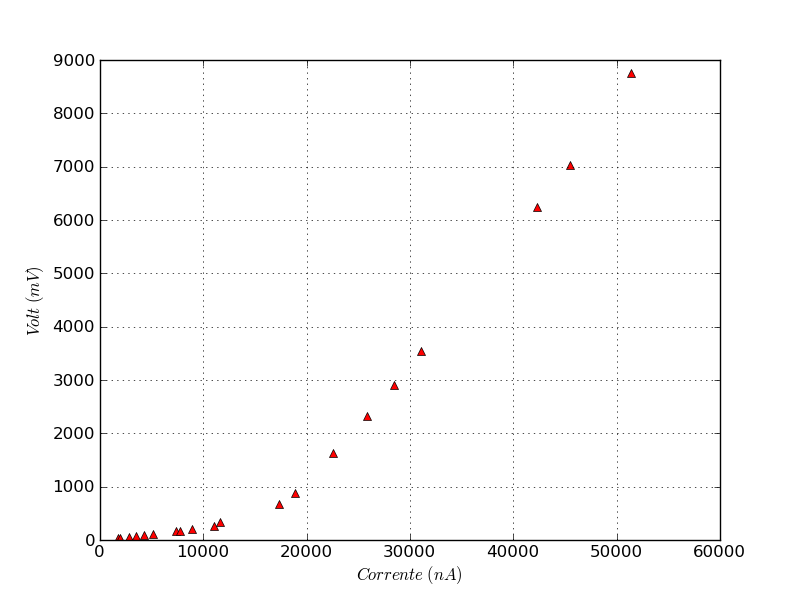
\includegraphics[scale=0.75]{grafici/C1/lampa.png}

La lampadina ha un comportamento non-ohmico nel momento in cui il filamento si scalda sufficientemente e inizia ad emettere luce ($500mV$).


\section{Partitore resistivo}

\subsection{Situazione senza carico}
\begin{center}
\begin{tabular}{*{2}{c}}
$V_{in}$ & $\frac{V_{in}}{V_{out}}$\\
\midrule
329.0 & 0.5015 \\
493.0 & 0.501 \\
544.0 & 0.5018 \\
618.0 & 0.5016 \\
667.0 & 0.5007 \\
776.0 & 0.5 \\
803.0 & 0.5006 \\
927.0 & 0.5005 \\
1078.0 & 0.5 \\
1285.0 & 0.4996 \\
\end{tabular}

\end{center}

$\chi^2=0.0169147373983$


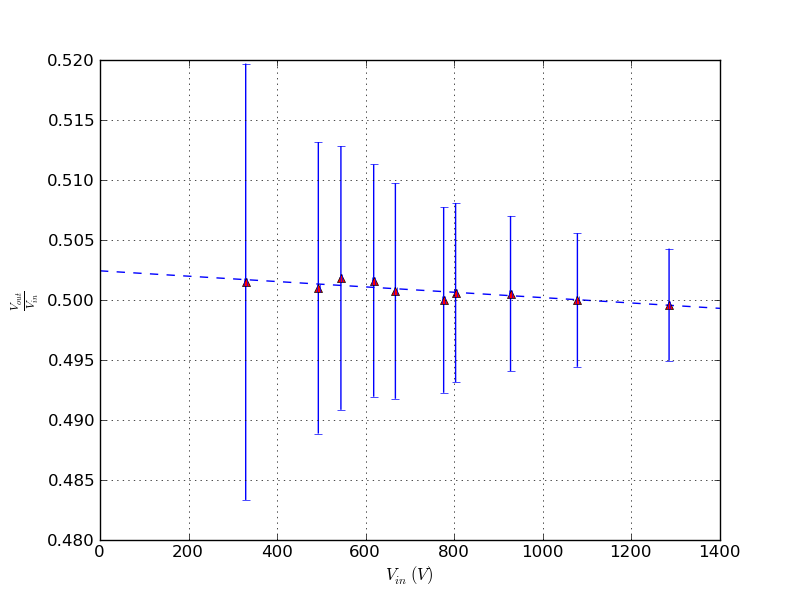
\includegraphics[scale=0.75]{grafici/C1/part1.png}

\subsection{Situazione con carico}
\begin{center}

\begin{tabular}{*{2}{c}}
$V_{in}$ & $\frac{V_{in}}{V_{out}}$\\
\midrule
220.0 & 3.1 \\
276.0 & 3.1051 \\
302.0 & 3.1126 \\
410.0 & 3.1073 \\
511.0 & 3.1115 \\
559.0 & 3.1055 \\
624.0 & 3.109 \\
752.0 & 3.109 \\
906.0 & 3.1093 \\
1036.0 & 3.111 \\
\end{tabular}

\end{center}
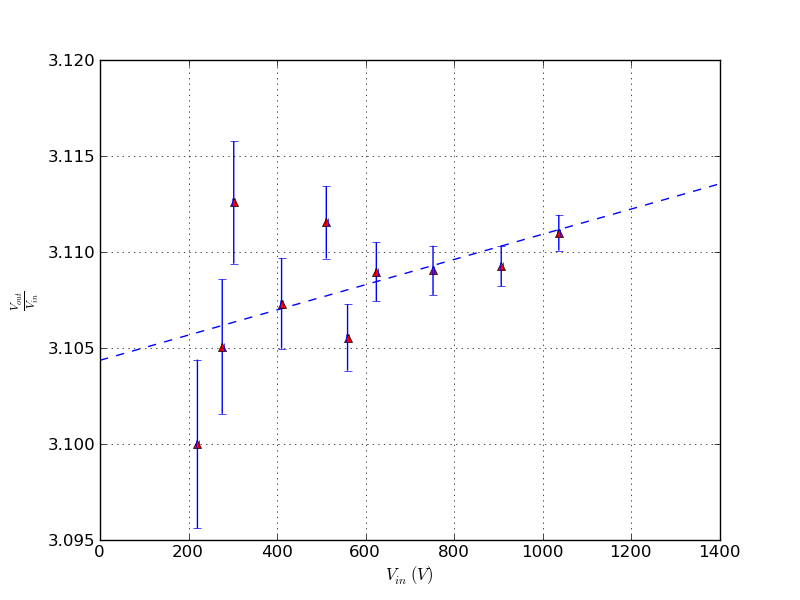
\includegraphics[scale=0.75]{grafici/C1/part2.png}

$\chi^2 = 12.9963702671$


\end{document} 



